\section{OPQ Box}
\label{sec:opq-box}

OPQ Box is a hardware device designed to provide inexpensive, extensible and accurate residential power quality measurements.
A block diagram of OPQ Box is shown in Figure~\ref{fig:opq:1:1}.
A complete device is shown in Figure~\ref{fig:opq:1:2}.

\begin{figure}[h]
	\centering
	\begin{subfigure}{.5\textwidth}
	  \centering
	  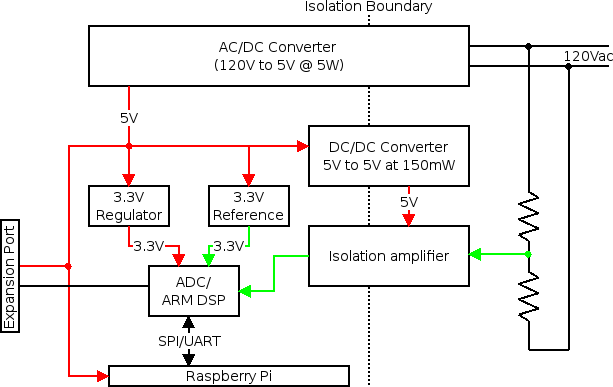
\includegraphics[width=0.9\linewidth]{images/opq-box/opqbox_diagram.png}
	  \caption{OPQ Box Block Diagram.
	  The power path is in red, signal path is in green and the digital IO is in black.}
	  \label{fig:opq:1:1}
	\end{subfigure}%
	\begin{subfigure}{.5\textwidth}
	  \centering
	  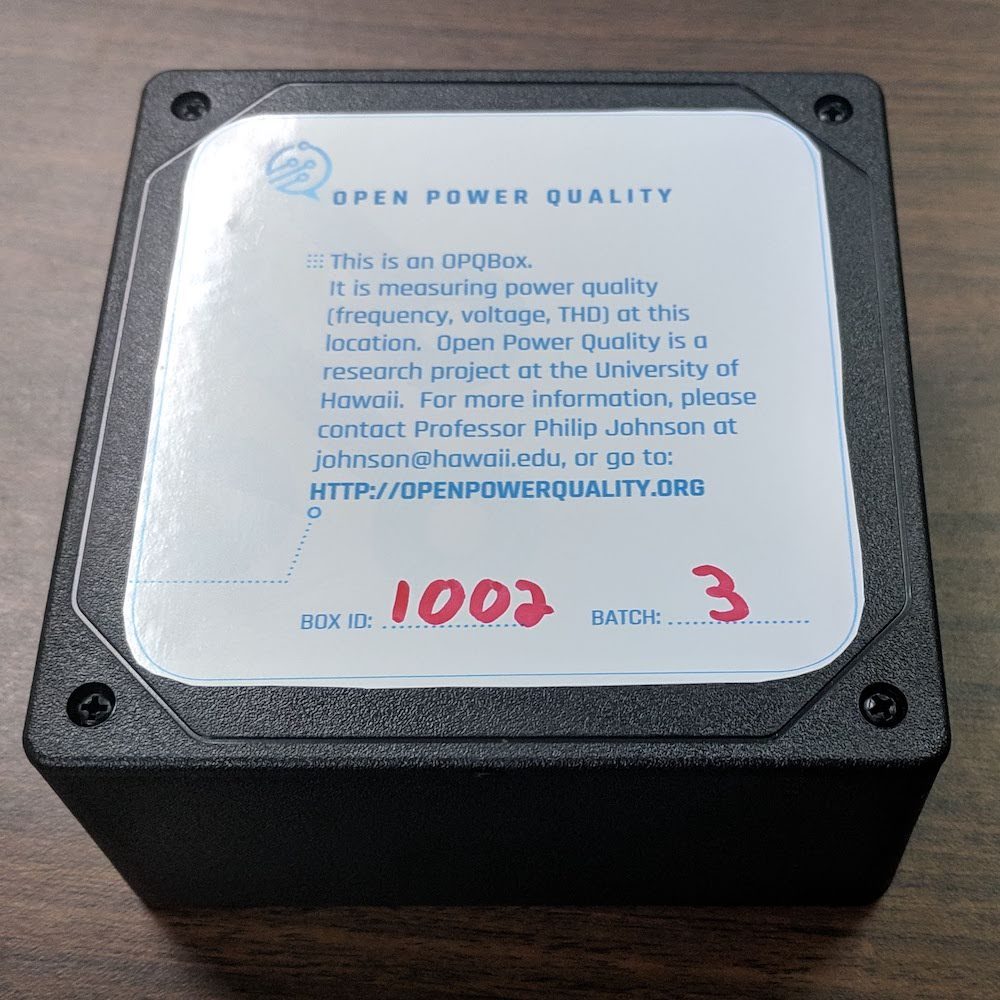
\includegraphics[width=0.7\linewidth]{images/opq-box/opqbox_photo.jpg}
	  \caption{OPQ Box in an ABS plastic enclosure.}
	  \label{fig:opq:1:2}
	\end{subfigure}
	\caption{(a) OPQ Box block diagram and (b) production OPQ Box ready for deployment}
	\label{fig:opq:2}
\end{figure}

\subsection{Hardware}\label{subsec:hardware}

The power system of the OPQ Box electrically isolates most of the device from the AC mains power.
An isolated AC-DC converter generates $5V_{dc}$ from the mains $120V_{ac}$.
5V is used to power the Raspberry Pi, the equipment connected to the expansion port, the 3.3V regulators and voltage reference and an isolated DC/DC converter.
3.3V is used to power the isolated end of the isolation amplifier as well as the STM32F3 analog to digital converter/digital signal processor (ADC/DSP).
The hot side of the isolation amplifier is powered from the isolated DC/DC converter.
This allows OPQ Box to function with a battery attached to the expansion port, so that it may retain data and continue to operate during a power outage.

The analog signal path of the OPQ Box is complicated by the fact that the STM32F3 ADC/DSP is electrically isolated from the mains power.
A previous iteration of the OPQ Box overcame this by employing a small circuit board mount isolation transformer.
Unfortunately it was found that the frequency response of these transformers varied wildly between individuals, thus incurring a lengthy calibration process for each device.
The current OPQ Box design solved this issue by using an AMC1100 isolation amplifier as the isolation component.
Internally, the AMC1100 consists of a single die comprised of a $\Sigma\Delta$ analog to digital and digital to analog converters.
These converters are separated by a silicon glass region on the integrated circuit which acts as a coupling capacitor.
Since the signal passes the isolation boundary as a $\Sigma\Delta$ encoded digital signal, it incurs no distortion and no additional calibration is required.
In order to match the dynamic range of the AMC1100, the $120V_{ac}$ is passed through the resistor divider to attenuate it to $120mV_{ac}$.
The input and output of the isolation amplifier is filtered with a passive first order anti-aliasing filter.
The isolated signal is then digitized via a 16bit ADC of the STM32F3 DSP at $12 KSps$, which gives 200 data samples per grid cycle.
Internally, the digitization process runs asynchronously with respect to the DSP CPU, in order to minimize timing jitter.
We verified that the sampling jitter of the ADC is less than 1us, however, due to the limited precision of our equipment, an exact figure was not established.
The data stream in its digital form is transferred to the Raspberry Pi single board computer (SBC) for analysis.

\begin{figure}[h]
  \begin{center}
  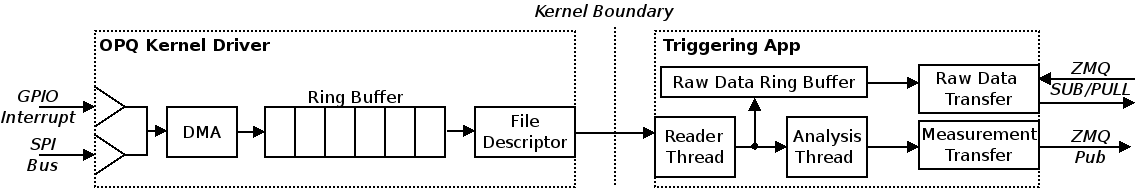
\includegraphics[width=0.9\textwidth]{images/opq-box/opqbox_software.png}
  \end{center}
  \caption{Block diagram of the OPQ Box 2 software stack.}
  \label{fig:opq:3}
\end{figure}

A Raspberry Pi single board computer (SBC) is responsible for signal analysis and anomaly detection.
The Raspberry Pi model used in OPQ Box is the Pi Zero W equipped with 256MB of main memory and a single core 1GHz ARM11 CPU. It also contains an on-board 802.11n WIFI transceiver, which removes the need for an external WIFI dongle.

\subsection{Software}\label{subsec:software}

The software stack of the Raspberry Pi aims to deliver an accurate and precise power quality analysis framework despite the rather limited capabilities of the hardware.
A block diagram of the software stack is shown in Figure~\ref{fig:opq:3}.
Digital data is transferred from the DSP to the Raspberry Pi via Serial Peripheral Interface, with the Pi acting as the master and the DSP as a slave device.
A hardware interrupt line is used to inform Pi software that the DSP is ready for the data transfer, and a kernel driver provides management of the SPI bus.
Internally, the OPQ driver maintains a ring buffer of 16 windows, each of which is 200 data samples in size.
Upon receiving the interrupt for the DSP, the CPU sets up the DMA transfer and the DMA engine transfers a 200 sample window into the kernel memory without CPU interaction.
This scheme requires the CPU to only service 60 interrupts a second, with each interrupt requiring on the order of 100 instructions, for a CPU utilization of less than $1\%$ in normal operation.
Userland applications communicate with the kernel driver using a file descriptor, where every $read$ system call yields 200 samples of raw waveform.
As a result, the smallest window that a userland application may process is a single AC cycle of the grid mains.

The userland component of the OPQ Box software is a multi-threaded extensible analysis framework called Triggering.
The reader thread is responsible for transferring and accumulating data from the kernel driver.
The smallest data buffer that the Triggering application processes at any given time is 10 grid cycles or 2k samples.
Once the cycles are transferred to the userland and timestamped, they are passed to the analysis thread for feature extraction, as well as to the Raw Data Ring Buffer (RDRB).
Since internally all data is addressed using shared pointers, during data duplication no copying is required.
RDRS is capable of buffering up to an hour of data before it is overwritten, resulting in the RDBS maximum size of 100MB.

The analysis thread of the Triggering application performs feature extraction of the raw data windows of 2000 samples.
Four metrics are extracted from the data stream: (1) Fundamental frequency, (2) RMS Voltage, (3) Total Harmonic Distortion, and (4) Transients. Let's briefly discuss how each of these are computed.

\subsubsection{Fundamental Frequency}\label{subsec:fundamental-frequency}

The fundamental frequency is calculated by computing the zero crossings of the AC waveform.
Since a sinusoid has two zero crossings for a full cycle, the frequency can be calculated as:
\begin{equation} \label{eq:1}
 f = \frac{1}{\frac{2}{n}\sum\limits_{k=0}^{k=n}{\Delta t_{k}}}
\end{equation}

\begin{figure}[ht!]
	\centering
	\begin{subfigure}{.8\textwidth}
	  \centering
	  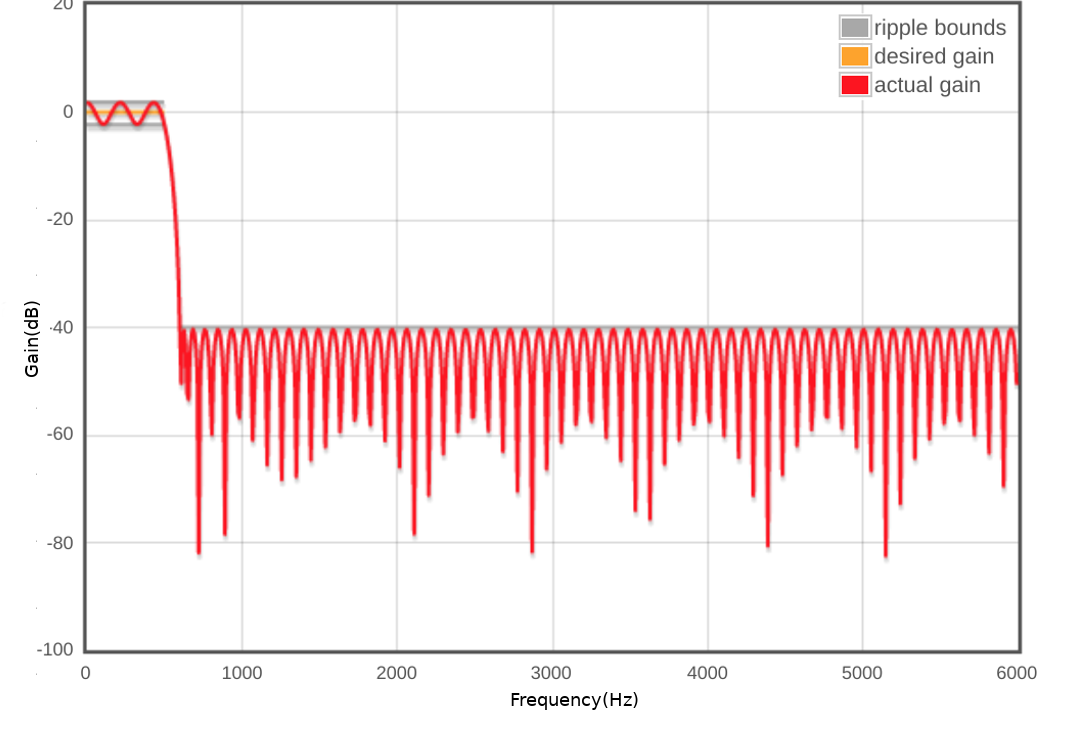
\includegraphics[width=1\linewidth]{images/opq-box/filter1_gain.png}
	  \caption{}
	  \label{fig:opq:4:1}
	\end{subfigure}%

	\begin{subfigure}{.8\textwidth}
	  \centering
	  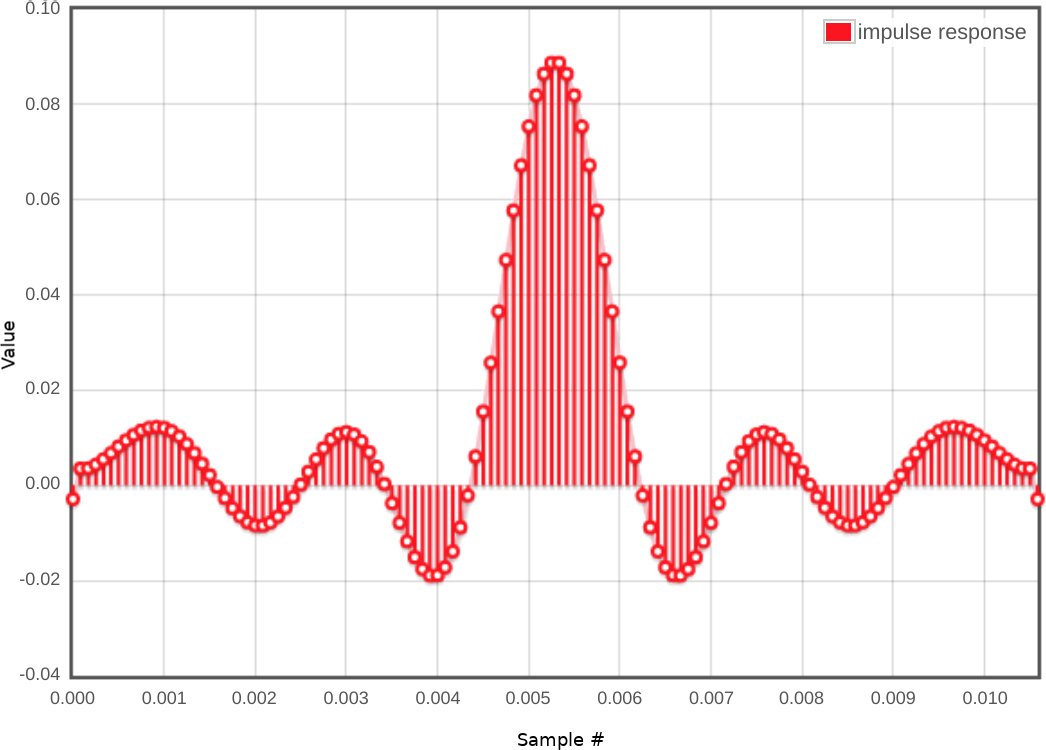
\includegraphics[width=1\linewidth]{images/opq-box/filter1_response.png}
	  \caption{}
	  \label{fig:opq:4:2}
	\end{subfigure}
\end{figure}
\begin{figure}[ht!]\ContinuedFloat
	\centering
	\begin{subfigure}{.75\textwidth}
	  \centering
	  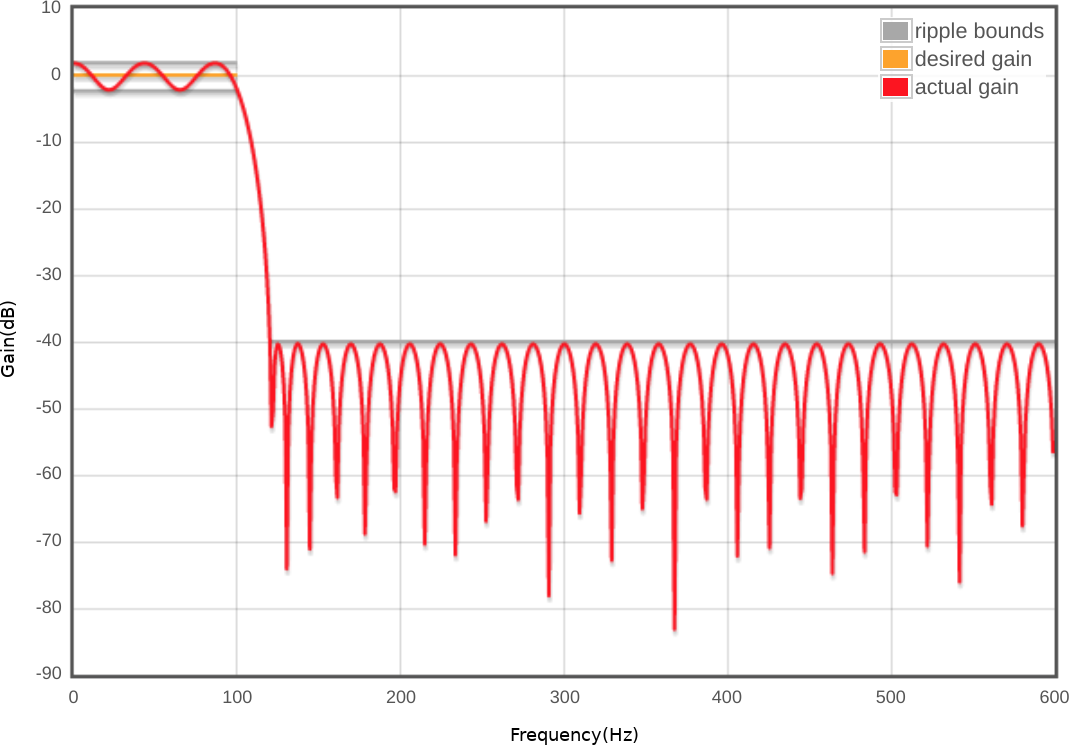
\includegraphics[width=1\linewidth]{images/opq-box/filter2_gain.png}
	  \caption{}
	  \label{fig:opq:4:3}
	\end{subfigure}%

	\begin{subfigure}{.75\textwidth}
	  \centering
	  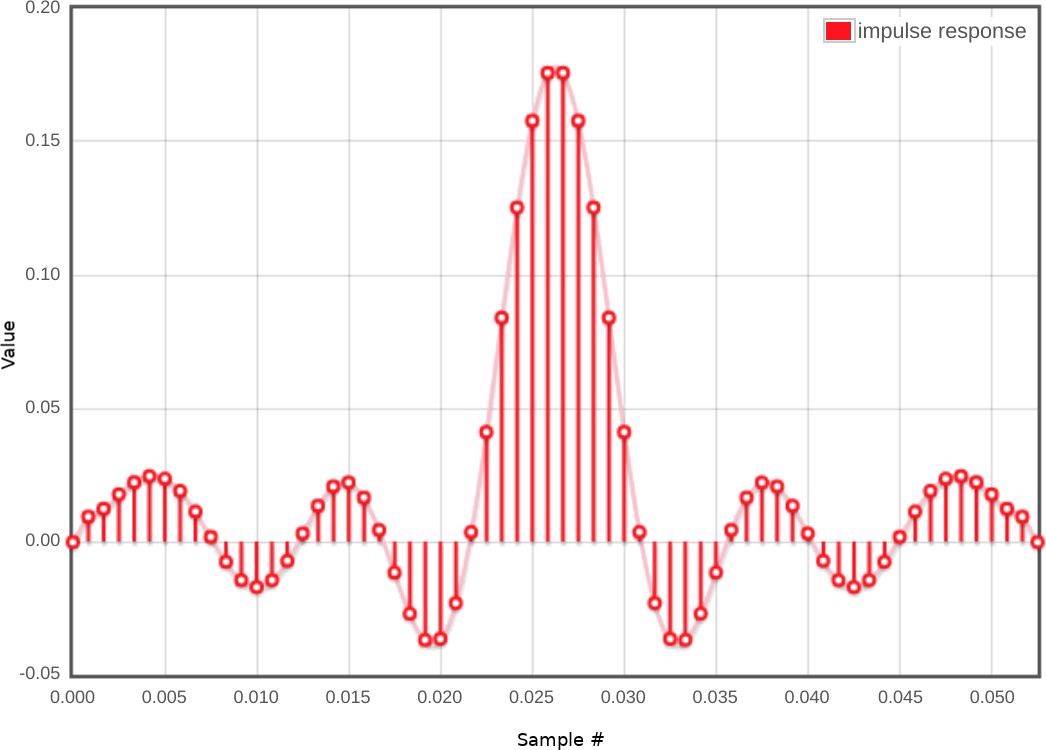
\includegraphics[width=1\linewidth]{images/opq-box/filter2_response.png}
	  \caption{}
	  \label{fig:opq:4:4}
	\end{subfigure}
	\caption{Filters used for mains frequency calculation. (a) Downsampling filter gain. (b) Downsampling filter impulse response. (c) Lowpass filter gain. (d) Lowpass filter impulse response.}
	\label{fig:opq:4}
\end{figure}

Where the $\Delta t_{k}$ is the k'th time between two adjacent zero crossings.

In order to improve the accuracy of the frequency calculation one must first filter out as much noise as possible.
Since our sampling rate is quite high (12kSps) and the fundamental frequency is quite low (60Hz), it is very computationally expensive to perform this filtering in a single step.
Instead, filtering is accomplished via a set of two finite impulse response (FIR) filters shown in Figure~\ref{fig:opq:4:2} and~\ref{fig:opq:4:4}.
First, the Down sampling filter is applied to the raw waveform, which results in the frequency response shown in Figure~\ref{fig:opq:4:1}.
As is evident by the plot, the frequency content of the result is 0-600Hz, Thus, it can be downsampled to the $\frac{N}{10}$, or 200 samples without aliasing.

Next, the low pass filter is applied to the downsampled waveform with the frequency response shown in Figure~\ref{fig:opq:4:3}.This resulting frequency content is 0-100Hz, thus all of the higher frequency harmonics and noise are removed.

Finally, the twice filtered downsampled waveform is used to estimate the fundamental frequency according to the Equation~\ref{eq:1}.
The zero crossings themselves were calculated by using linear interpolation between two points which bracket the time axis.

\subsubsection{Root Mean Square Voltage}\label{subsec:root-mean-square-voltage}

Root mean square voltage ($V_{rms}$) in electrical power is the equivalent value of DC voltage which would dissipate the same power in the resistive load. $V_{rms}$ is a convenient measure for detecting voltage sags and swells, since they result in nominally higher and lower computed value.
For a sinusoidal signal, $V_{rms}$ can be calculated from the peak to peak value ($V_{pp}$) as:
\begin{equation} \label{eq:2}
	V_{rms} = \frac{V_{pp}}{2\sqrt{2}}
\end{equation}
It is common for multimeters to employ the equation above for computing $V_{rms}$.
However, this equation is only valid for a perfect sinusoid, and thus does not result in a suitable metric for identifying power quality disturbances.
Instead, OPQ Box computes $V_{rms}$ as follows:
\begin{equation} \label{eq:3}
	V_{rms} = \sqrt{\frac{1}{n}\sum\limits_{k=0}^{k=n}V_{k}^{2}}
\end{equation}
Similarly to the frequency calculation, OPQ Box uses a 10 cycle window for a single $V_{rms}$ calculation, however unlike the frequency calculation the input is not filtered a priori.

An example of a power quality disturbance which exhibits low $V_{rms}$ is shown in Figure~\ref{fig:opq:6:1} and~\ref{fig:opq:6:2}.
These disturbances are the result of a lighting strike recorded by two OPQ Box devices on Nov 1, 2017.

\begin{figure}[h]
		\centering
	\begin{subfigure}{.5\textwidth}
	  \centering
	  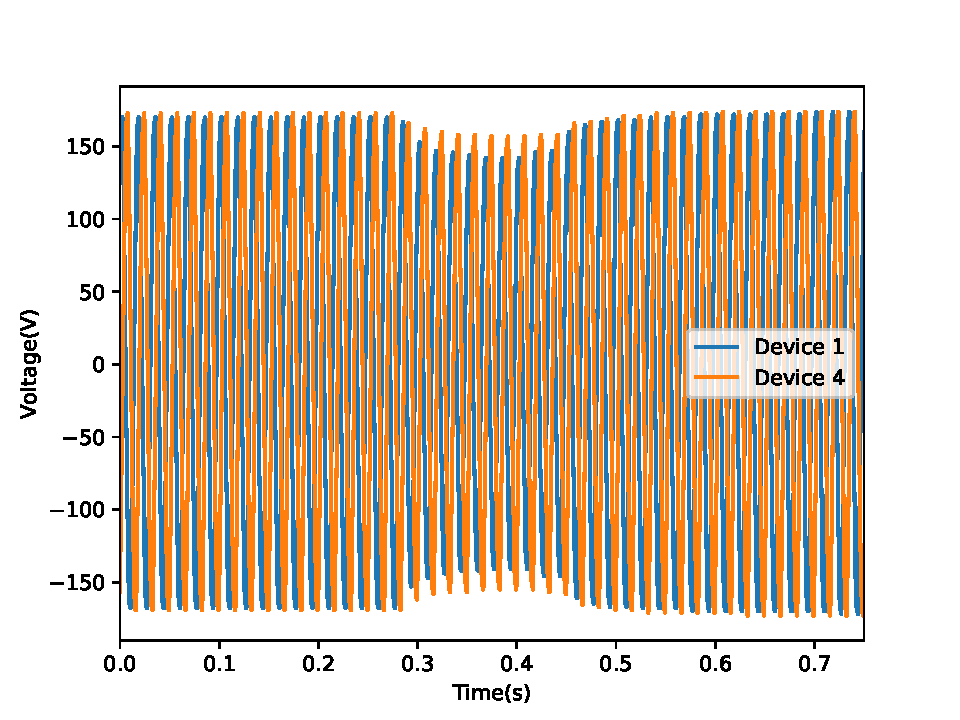
\includegraphics[width=0.9\linewidth]{images/opq-box/voltage_sag.pdf}
	  \caption{}
	  \label{fig:opq:6:1}
	\end{subfigure}%
	\begin{subfigure}{.5\textwidth}
	  \centering
	  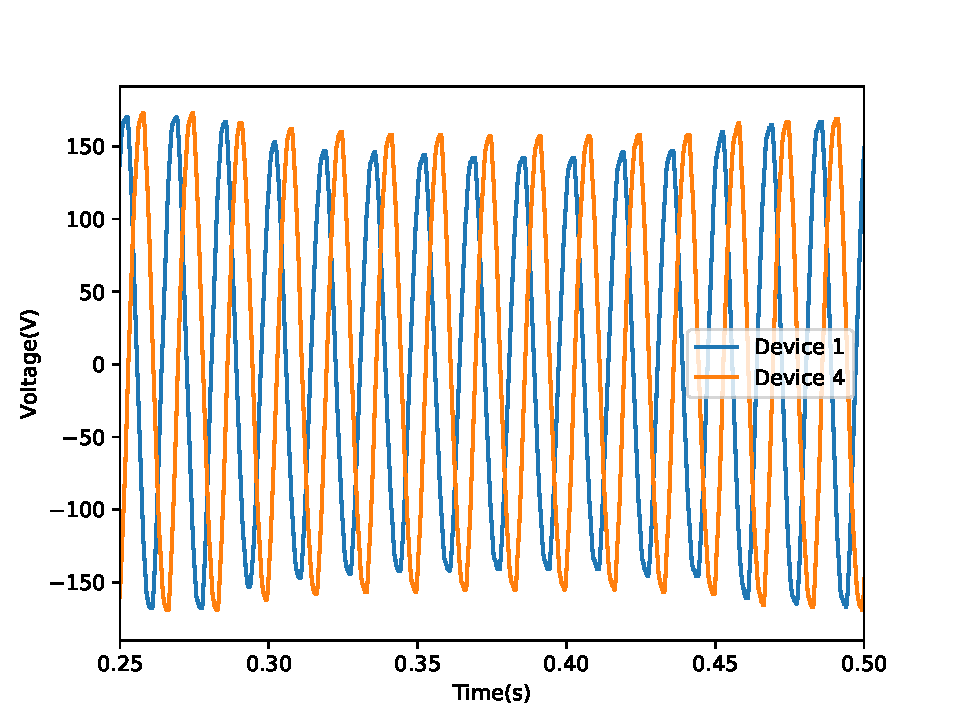
\includegraphics[width=0.9\linewidth]{images/opq-box/voltage_sag_zoomed_in.pdf}
	  \caption{}
	  \label{fig:opq:6:2}
	\end{subfigure}
	\caption{A lightning strike recorded by two OPQ Box 2 devices separated by 10 miles. (a) A lightning strike manifested as a $V_{rms}$ dip which lasted 11 cycles. (b) As a consequence of using NTP these devices have a $\frac{1}{2}$ cycle mismatch in reported timestamps.}
	\label{fig:opq:6}
\end{figure}


\subsubsection{Total Harmonic Distortion}\label{subsec:thd}

The OPQ Box calculates total harmonic distortion (THD) using the industry standard methodology.
In the power delivery industry, THD is defined as:
\begin{equation} \label{eq:4}
THD = \frac{\sqrt{\sum{V_{n}^2}}}{V_{f}}*100\%
\end{equation}
Where $V_{f}$ is the fundamental 60Hz power and $V_{n}$ is the power at $n^{th}$ harmonic.

It should be noted that in the power quality domain THD is expressed as a percentage as opposed to $\frac{dB}{\sqrt{Hz}}$ as used in other disciplines.
Operationally, OPQ Box computes THD for 10 cycles of the fundamental frequency.
First an FFT transforms the real voltage samples into its frequency components.
Next, the square of the harmonic bins is accumulated and scaled by the magnitude of the fundamental power.

\begin{figure}[h]
	\centering
	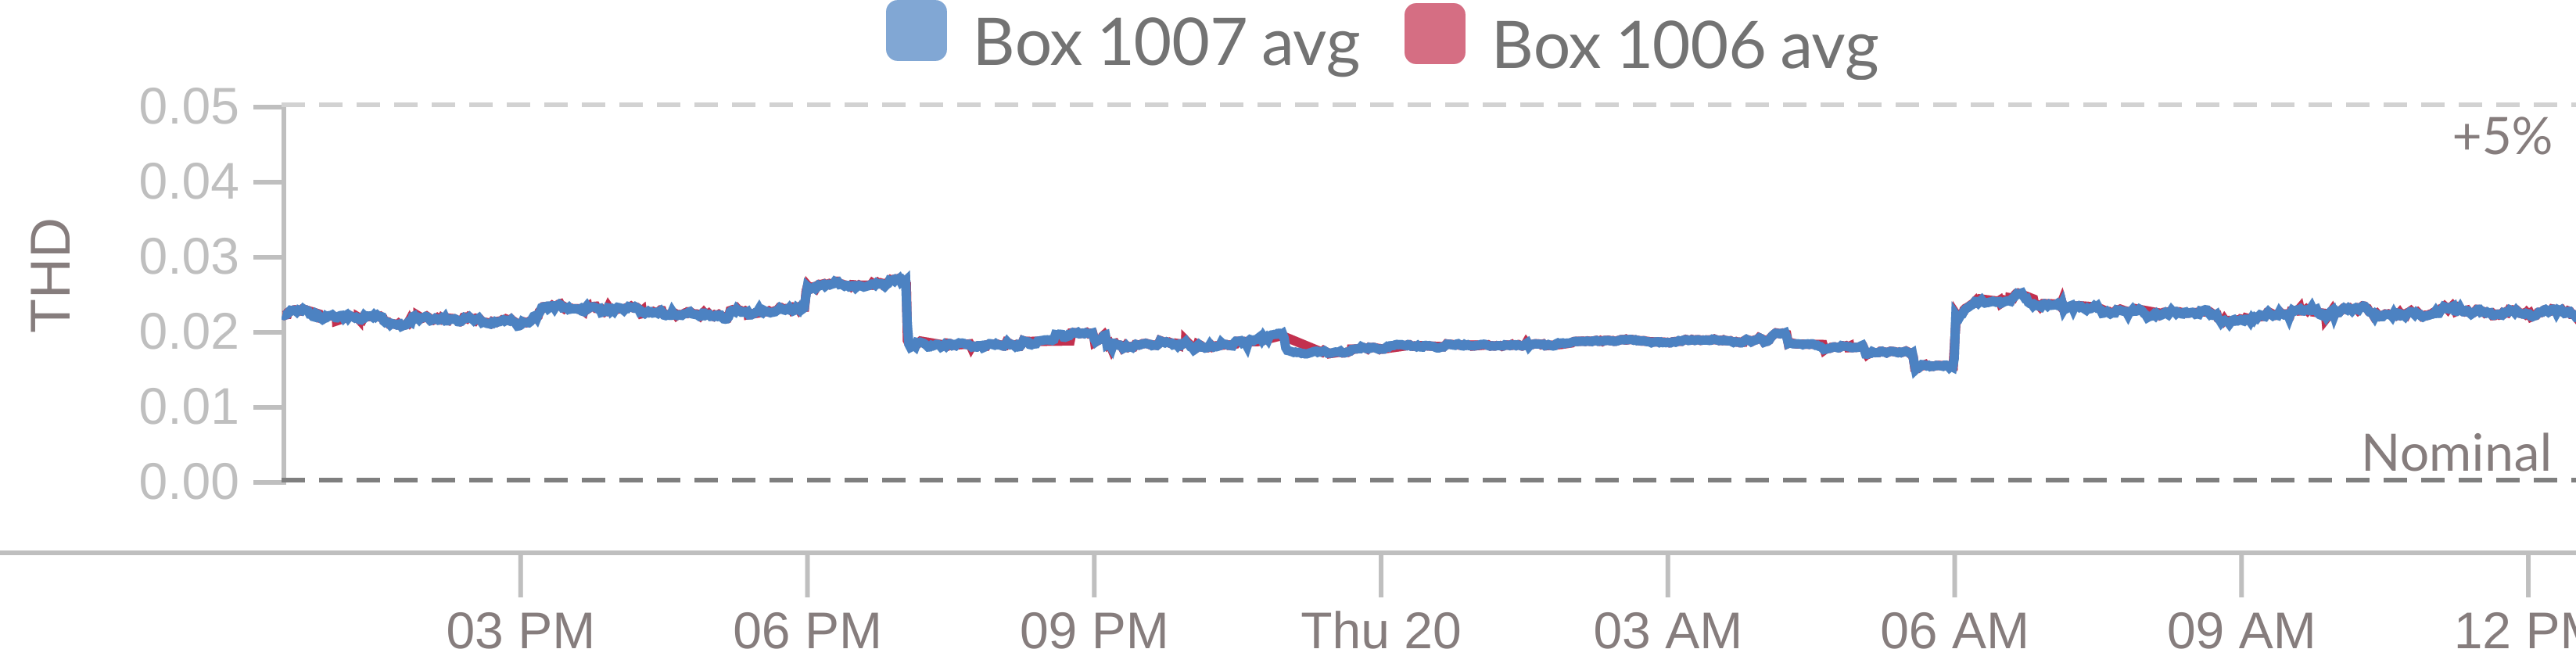
\includegraphics[width=1\linewidth]{images/opq-box/thd_two_devices_24_hours.png}
	\caption{A common THD trend across two OPQ Box devices deployed in two buildings on the University of Hawaii campus.}
	\label{fig:opq:7}
\end{figure}

Figure~\ref{fig:opq:7} shows a common trend observed by OPQ Box devices installed on the UH campus.
For clarity, only two devices are shown.
It is assumed that the large drop observed daily from approximately 6pm to 6am corresponds to the automatic response of the power delivery system to the reactive power in the grid, by deploying a large capacitor bank to compensate for the current phase lag.

\subsubsection{Transient Detection}\label{subsec:transient-detection}

OPQ Box transient detection is performed via filtering out of the fundamental frequency via an FIR high pass pass filter and searching for a maximum value in the remainder.
The high pass filter has a cutoff of $400Hz$, and the filter coefficients and response are shown in Figure~\ref{fig:opq:8:2} and Figure~\ref{fig:opq:8:1} respectively.
The result of the high pass filter operation is shown in Figure~\ref{fig:opq:8}.
Figure~\ref{fig:opq:8:3} shows a synthetic signal generated via a SDG1025 signal generator and fed into the OPQ Box.
This signal contains a $5V_{pp}$ transient injected at 11ms.
The filtered signal is shown in Figure~\ref{fig:opq:8:4}, with the fundamental removed and the transient preserved.
OPQ Box scans for the highest sample in the filtered waveform and uses its magnitude as a transient detection metric.


\begin{figure}[h]
	\centering
	\begin{subfigure}{.5\textwidth}
		\centering
		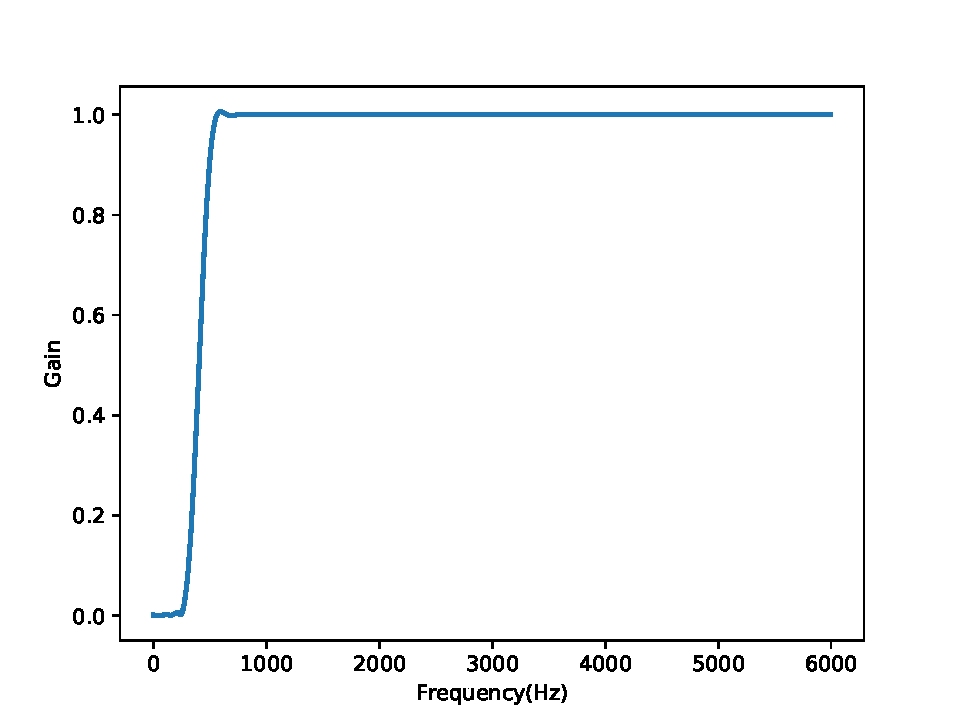
\includegraphics[width=1\linewidth]{images/opq-box/thd_hpf_resp.pdf}
		\caption{}
		\label{fig:opq:8:1}
	\end{subfigure}%
	\begin{subfigure}{.5\textwidth}
		\centering
		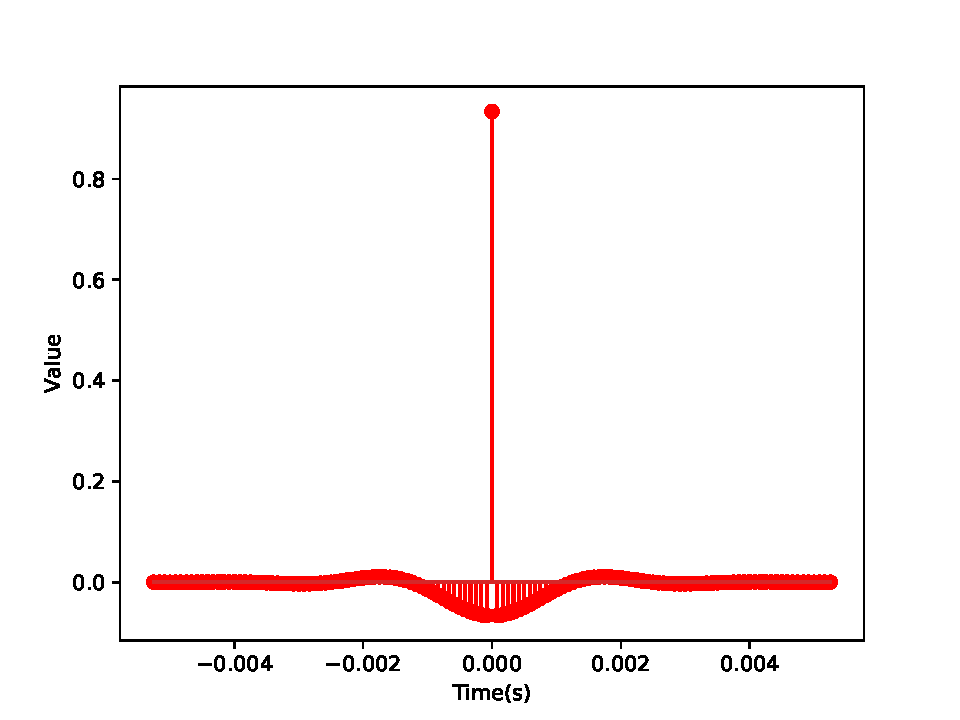
\includegraphics[width=1\linewidth]{images/opq-box/thd_hpf.pdf}
		\caption{}
		\label{fig:opq:8:2}
	\end{subfigure}

	\begin{subfigure}{.5\textwidth}
		\centering
		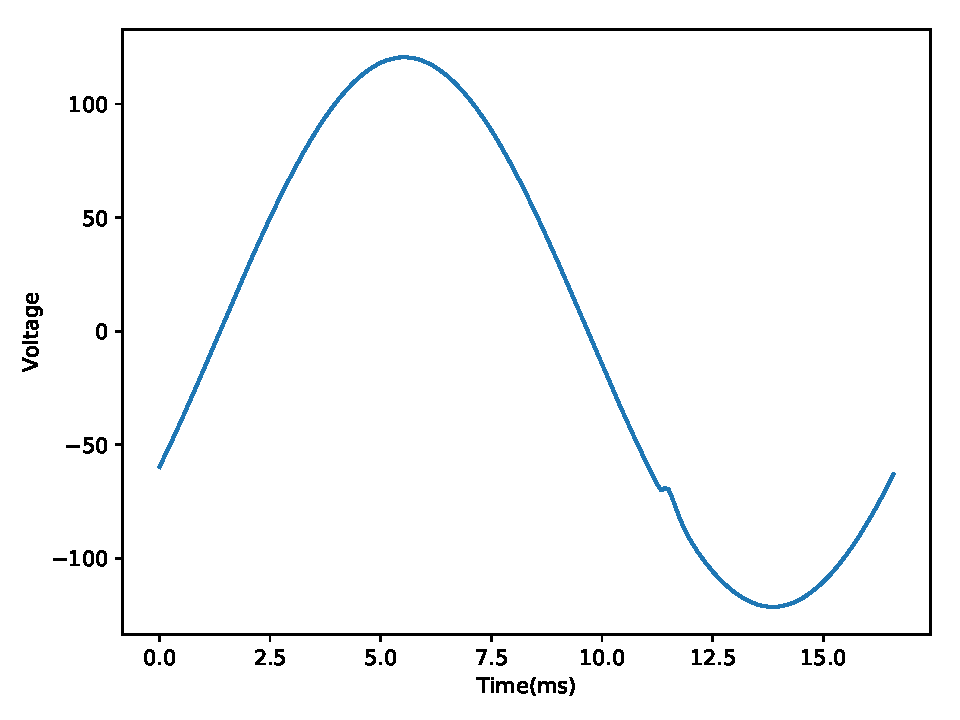
\includegraphics[width=0.86\linewidth]{images/opq-box/box_eval/5v_transient.pdf}
		\caption{}
		\label{fig:opq:8:3}
	\end{subfigure}%
	\begin{subfigure}{.5\textwidth}
		\centering
		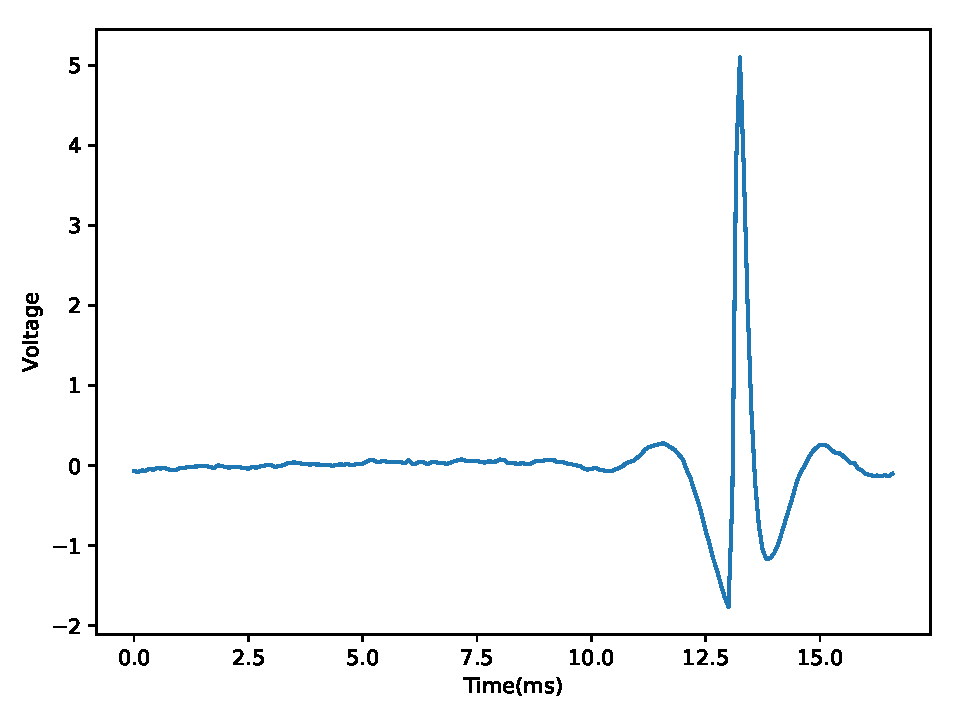
\includegraphics[width=0.86\linewidth]{images/opq-box/box_eval/5v_transient_filtered.pdf}
		\caption{}
		\label{fig:opq:8:4}
	\end{subfigure}
	\caption{THD detection filtering. (a) Filter gain. (b) Filter response. (c) A 5V transient superimposed onto a fundamental. (d) Filter result from (c).}
	\label{fig:opq:8}
\end{figure}

It should be noted that this transient detection method is susceptible to THD fluctuations, since any harmonic above $400Hz$ will remain in the filtered waveform.
However, since the THD information is transmitted along with the transient detection metric, they can be correlated in downstream transient detection.
This effect can be seen in Figure~\ref{fig:opq:9}.
This figure shows both the THD and transient detection metric during a transient event.
A small transient of approximately 1.6V was observed occurring at 2600s, while the sensitivity of the transient metric is clearly visible, particularly between 3000s and 4500s.

\begin{figure}[h]
	\begin{center}
		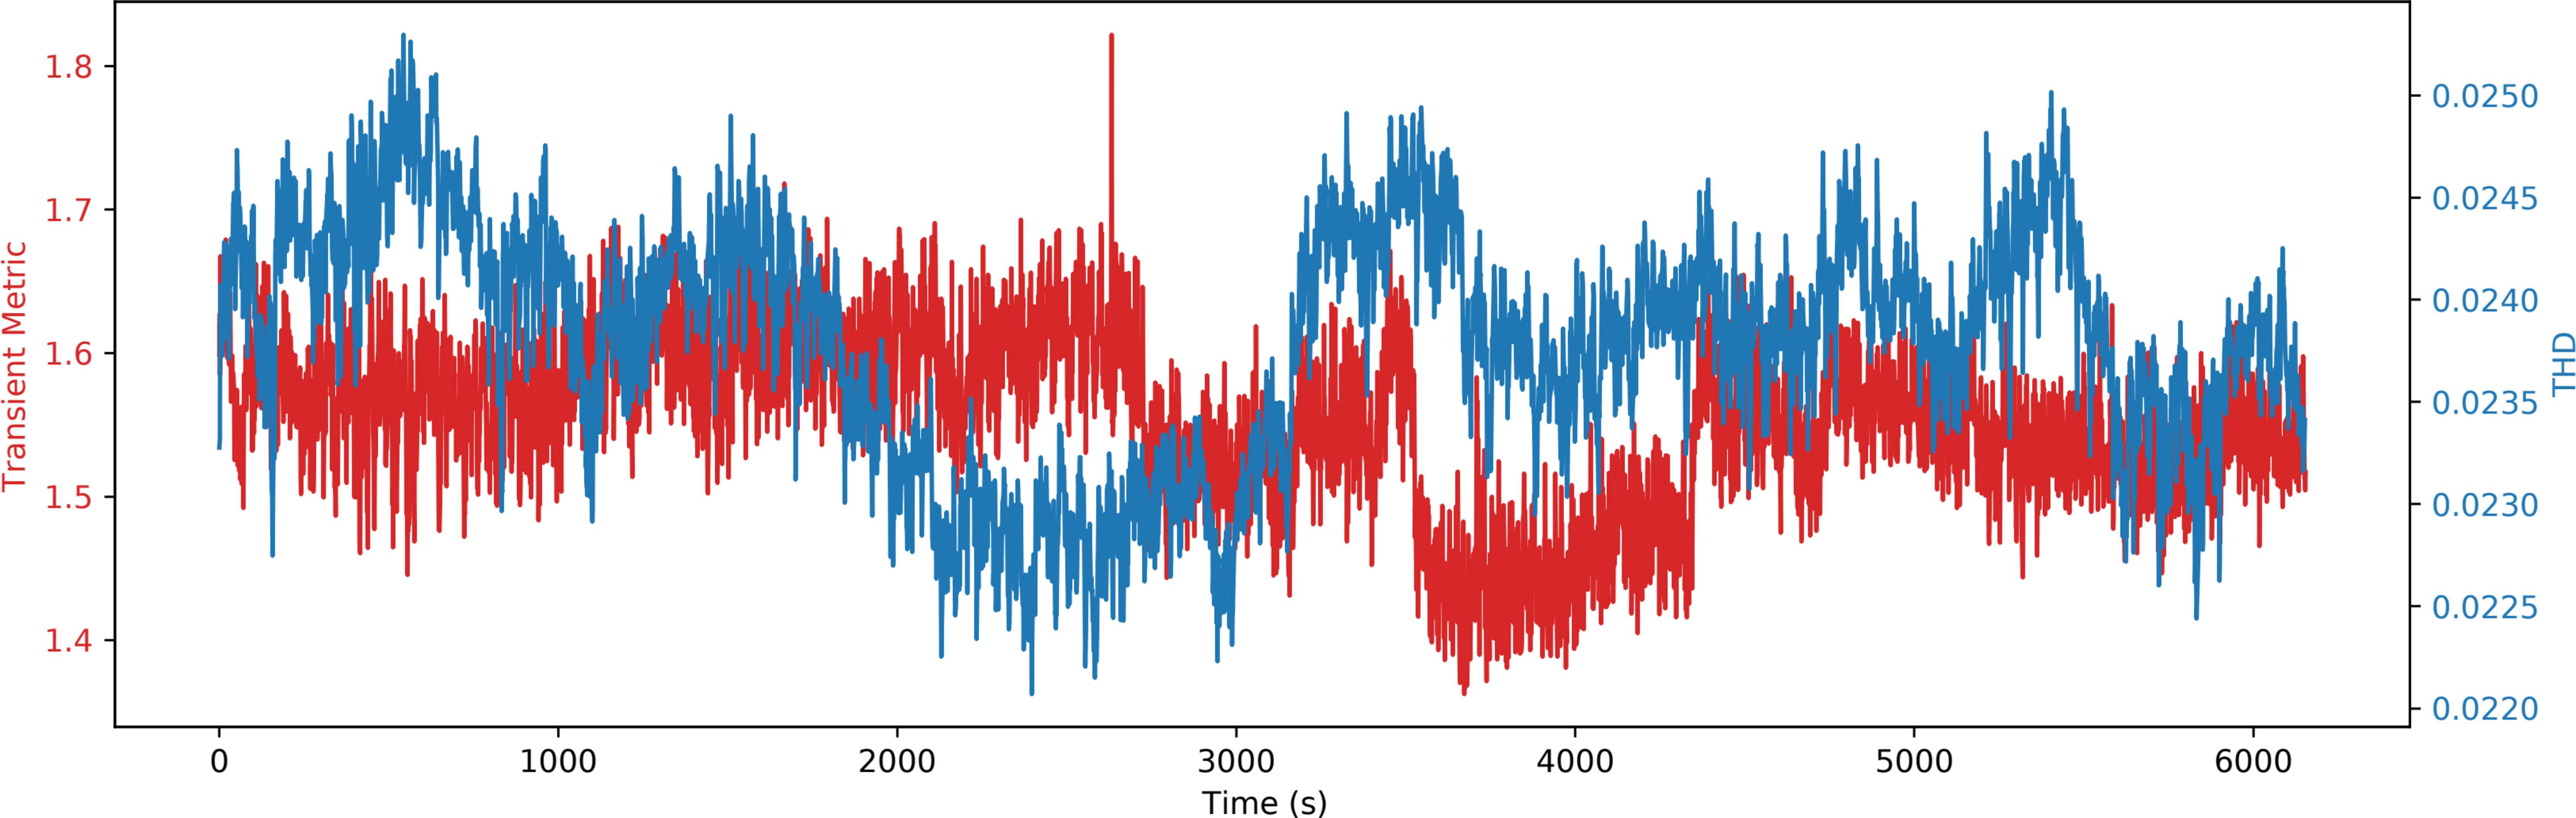
\includegraphics[width=1\textwidth]{images/opq-box/trans_thd_det.pdf}
	\end{center}
	\caption{THD and Transient detection metric.}
	\label{fig:opq:9}
\end{figure}

\subsubsection{Network Communication}\label{subsec:network-communication}

The computed fundamental frequency and $V_{rms}$ are transmitted to the Makai service for aggregation.
Data transmission is handled using ZeroMq software stack with Curve25519 elliptic curve encryption.
Each device holds a unique private and public key, as well as the servers' public key, allowing both the Makai service and the OPQ Box to verify its peer.
Internally, metrics transmission uses ZeroMq's PUB/SUB protocol.
This protocol is a publish subscribe topology, with each message containing the topic, and a payload.
Additionally, ZeroMq allows for multiple sub peers with subscriptions forwarded to the publisher automatically via a side channel.
This allows for the aggregation service to be spread across multiple nodes, with minimal network overhead.

If the aggregation service determines that an anomaly has occurred, it is able to request raw waveform from the OPQ Box RDRB via a separate ZeroMq pub sub channel.
If the RDRB buffer contains data for the requested temporal range, OPQ Box transmits the available data to the aggregation service via a push pull ZeroMq channel.
Protobuf message serialization is used to encode messages across the OPQ ecosystem.


In order to make a distributed measurement, all of the OPQ Boxes on the OPQ network need to maintain an accurate time reference.
Time synchronization across multiple OPQ Boxes is accomplished using the Network Time Protocol.
The expansion port of the OPQ Box supports a GPS receiver.
However, since GPS receivers require line of sight to the sky, it was not used for deployment.
NTP performance has been verified against GPS resulting in time error of $8ms\pm 5ms$ which is typical for NTP running over the Internet with a close by NTP server.
This error is visualized in a Figure~\ref{fig:opq:6:2}.
With a large coincidental $V_{pp}$ drop across two devices, a 7ms phase error is clearly visible.

